% This is samplepaper.tex, a sample chapter demonstrating the
% LLNCS macro package for Springer Computer Science proceedings;
% Version 2.20 of 2017/10/04
%
\documentclass[runningheads]{llncs}
%
\usepackage{cite,url,amsfonts}
\usepackage{algorithm}% http://ctan.org/pkg/algorithms
\usepackage{algpseudocode}% http://ctan.org/pkg/algorithmicx
\usepackage{mathtools}
\usepackage{graphicx}
\usepackage{color}
\usepackage{hyperref}
% Used for displaying a sample figure. If possible, figure files should
% be included in EPS format.
%
% If you use the hyperref package, please uncomment the following line
% to display URLs in blue roman font according to Springer's eBook style:
% \renewcommand\UrlFont{\color{blue}\rmfamily}

\graphicspath{{figs/}, {../figures/}}

\begin{document}
%
\title{Artistic Curve Steganography Carried by Musical Audio}
%
%\titlerunning{Abbreviated paper title}
% If the paper title is too long for the running head, you can set
% an abbreviated paper title here
%
\author{First Author\inst{1}\orcidID{0000-1111-2222-3333}}
%
\authorrunning{F. Author et al.}
% First names are abbreviated in the running head.
% If there are more than two authors, 'et al.' is used.
%
\institute{Princeton University, Princeton NJ 08544, USA 
\email{lncs@springer.com}}
%
\maketitle              % typeset the header of the contribution
%
\begin{abstract}
The abstract should briefly summarize the contents of the paper in
15--250 words.

\keywords{Steganography, Traveling Salesperson Art, Hidden Signals}
\end{abstract}
%
%
%
\section{Introduction}



Our goals and design constraints are as follows:
\begin{enumerate}
    \item \label{goal:imperceptible} The hidden data should be audibly imperceptible
    \item \label{goal:geomquality} The hidden data should be faithfully preserved and {\em robust to compression}
    \item \label{goal:nokeys} It should be possible to decode the data without any prior knowledge/keys
    \item \label{goal:misalignment} The hidden data should be robust to frame misalignment, or it should be possible to recover a frame alignment without any prior information
    \item \label{goal:partial} It should be possible to recover the data partially from partial audio chunks; that is, we don't need to wait for the entire data stream to recover the signal
\end{enumerate}

Goals ~\ref{goal:imperceptible} and ~\ref{goal:geomquality} are at odds with each other, and satisfying them simultaneously is the biggest challenge of this work.

Pipeline is simple enough that we have very good intuition for how it's working, and we validate its performance in Section~\ref{sec:experiments}.


\subsection{Prior Work in Audio Steganography}

\section{Traveling Salesperson Art}

\begin{figure}
  \centering
  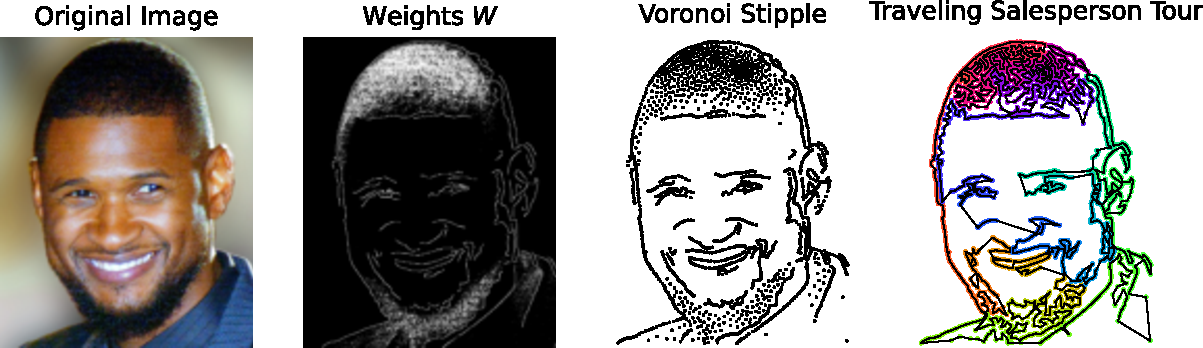
\includegraphics[width=\columnwidth]{TSPTour.pdf}
  \caption{Our modified pipeline for creating TSP art.  Color on the tour indicates phase along the loop.}
  \label{fig:TSPTour}
\end{figure}

Traveling Salesperson (TSP) art \cite{bosch2004continuous, kaplan2005tsp,bosch2008connecting} is an automated artistic line drawing pipeline which computes a {\em simple closed loop} to approximate a source image.  ``Simple'' in this context does not imply a lack of complexity; rather, it means that a curve does not intersect itself (see, for example, the Jordan Curve Theorem \cite{bosch2009jordan}).  To construct such a curve, we first place a collection of dots in the plane in a ``stipple pattern'' to approximate brightness in the image (e.g. more dots concentrate in darker regions), and then connect them in a loop via an approximate traveling salesperson (TSP) tour.  Figure~\ref{fig:TSPTour} shows an example.  We follow the TSP Art technique of \cite{kaplan2005tsp}, with a few modifications, as described below.


\subsection{Voronoi Stippling}
\label{sec:stippling}

\begin{algorithm}
  \caption{Modified Weighted Voronoi Stippling \cite{secord2002weighted}}
  \begin{algorithmic}[1]
    \Procedure{VoronoiStipple}{$G$, $N$, $b$, $\sigma$, $f$}
    \Comment{Grayscale image $G$, $N$ target points, brightness threshold $b$, Canny edge scale $\sigma$, density factor $f$}
    \State $W_{ij} \gets \min(I_{ij}, b)$
    \State $W_{ij} \gets W_{ij} - \min(W)$
    \State $W_{ij} \gets 1 - W_{ij} / \max(W)$
    \State $C \gets \text{canny}_{\sigma}(I)$ \Comment{1 if on canny edge, 0 otherwise}
    \State $W_{ij} \gets \max(W_{ij}, C_{ij})$
    \State  Sample $N$ random points $X \in \mathbb{R}^{N \times 2}$ by density according to $W$
    \For{$k = 1:10$} \Comment{Lloyd's relaxation iterations}
        \State \begin{equation}
          X_i \gets \frac{ \sum_{(i, j) \in A_i} W_{ij} * (i, j) }{\sum_{(i, j) \in A_i} W_{ij}}
        \end{equation}
        \Comment{Where $A_i$ is the Voronoi region for point $X_i$}
    \EndFor \\
    \State Remove top $N(1-f)$ points from $X$ with furthest distance to their nearest neighbors \\
    \Return $X$
    \EndProcedure
  \end{algorithmic}
  \label{alg:voronoistipple}
\end{algorithm}

%\begin{algorithm}
%  \caption{2-Opt Approximate TSP Tour \cite{johnson1997traveling}}
%  \begin{algorithmic}[1]
%    \Procedure{TSP2Opt}{$X$}
%    \Comment{$X \in \mathbb{R}^{N \times 2}$ is a 2D point cloud}
%    \State Let $T$ be a minimum spanning tree of $X$
%    \State Let $tour$ be indices into $X$ in the order that a depth-first search visits $T$, starting at an arbitrary point
%    \While{There exits a swappable $i > 1$, $j > i$}
%      \State Reverse indices in $tour$ in $[i+1, j]$
%    \EndWhile \\
%    \EndProcedure
%  \end{algorithmic}
%  \label{alg:twoopt}
%\end{algorithm}

The first step in TSP art is to generate a stipple pattern $X$ to best approximate a grayscale image $G$.  Following the authors of \cite{kaplan2005tsp}, we use Secord's technique for Voronoi stippling \cite{secord2002weighted}.  This consists taking an initial sample of points according to some density weights $W$ and then repeatedly moving them closer the weighted centroid of their Voronoi regions (an instance of Lloyd's algorithm) so that they are spread more evenly and look less ``noisy.''  Secord \cite{secord2002weighted} takes the weight $W_{ij}$ at a pixel to be inversely proportional to its brightness, using a weight of $0$ above some brigtness threshold $b$.  This leads more dots to concentrate in darker regions; however, the algorithm may fail to sample any dots along important edges between brighter regions (the authors of \cite{li2011structure} also observed this).   To ameliorate this, we run a Canny edge detector \cite{canny1986computational} on the original image and set the weight of any pixels along an edge to be 1, so that the final weights promote samples both in darker regions and along edges of any kind.  This addition is particularly helpful for line drawings, including images with text (e.g. Figure~\ref{fig:caltech101examples}).  Finally, we include the option to filter out points by density to clean up the stipple before the next step.  Algorithm~\ref{alg:voronoistipple} provides more details.

\subsection{Traveling Salesperson Tours}
\label{sec:tsp}
Once a stipple has been established, the next step in TSP art is to ``connect the dots'' with a closed loop that visits each stipple point exactly once, referred to as a ``tour''\footnote{A loop with these properties is otherwise known as a {\em Hamiltonian cycle} on a complete graph over the points}.  A well known objective function for a tour that doesn't ``jump too much'' is the total distance traveled, or the sum of all edge lengths, and a tour that achieves the optimum is known as a {\em traveling salesperson (TSP) tour}.  Since the TSP problem is NP-hard, the authors of  \cite{kaplan2005tsp} use the Concorde TSP solver \cite{applegate2001concorde} for an approximate solution. We opt for a simpler technique that first creates a 2-approximation of a TSP from a depth-first traversal through the minimum spanning tree of the stipple dots, which is a already a 2-approximation of the optimal tour.  We then iteratively improve on this tour via a sequence of 2-opt relaxations \cite{johnson1997traveling}; that is, if for some $i > 1, i < j < N$ the distances between the 4 points $X_i, X_{i+1}, X_j$, and $X_{j+1}$ satisfy

\begin{figure}
  \centering
  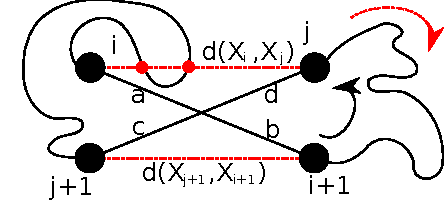
\includegraphics[width=0.5\columnwidth]{2Opt.pdf}
  \caption{Every crossing in a tour can be removed with a 2-opt swap to yield a tour of a smaller distance, since, by the triangle inequality, $d(X_i, X_j) + d(X_{i+1}, X_{j+1}) < (a+d) + (b+c) = d(X_i, X_{i+1}) + d(X_j, X_{j+1})$.  This may introduce new crossings (shown in red), but these and other crossings will be resolved in future 2-opt swaps.}
  \label{fig:TwoOpt}
\end{figure}

\begin{equation}
  d(X_i, X_j) + d(X_{i+1}, X_{j+1}) < d(X_i, X_{i+1}) + d(X_j, X_{j+1})
\end{equation}

then it is possible to perform a swap to yield a new tour with a smaller distance.  This amounts to reversing the indices in the tour between index $i+1$ and $j$, inclusive.  We repeat this step as long as such a swap is still possible.  Though this is not guaranteed to yield an optimal TSP tour, it does produce tours which are simple; that is, every crossing is removed (Figure~\ref{fig:TwoOpt}).


\subsection{Curvature Shortening Flow}

\begin{figure}
  \centering
  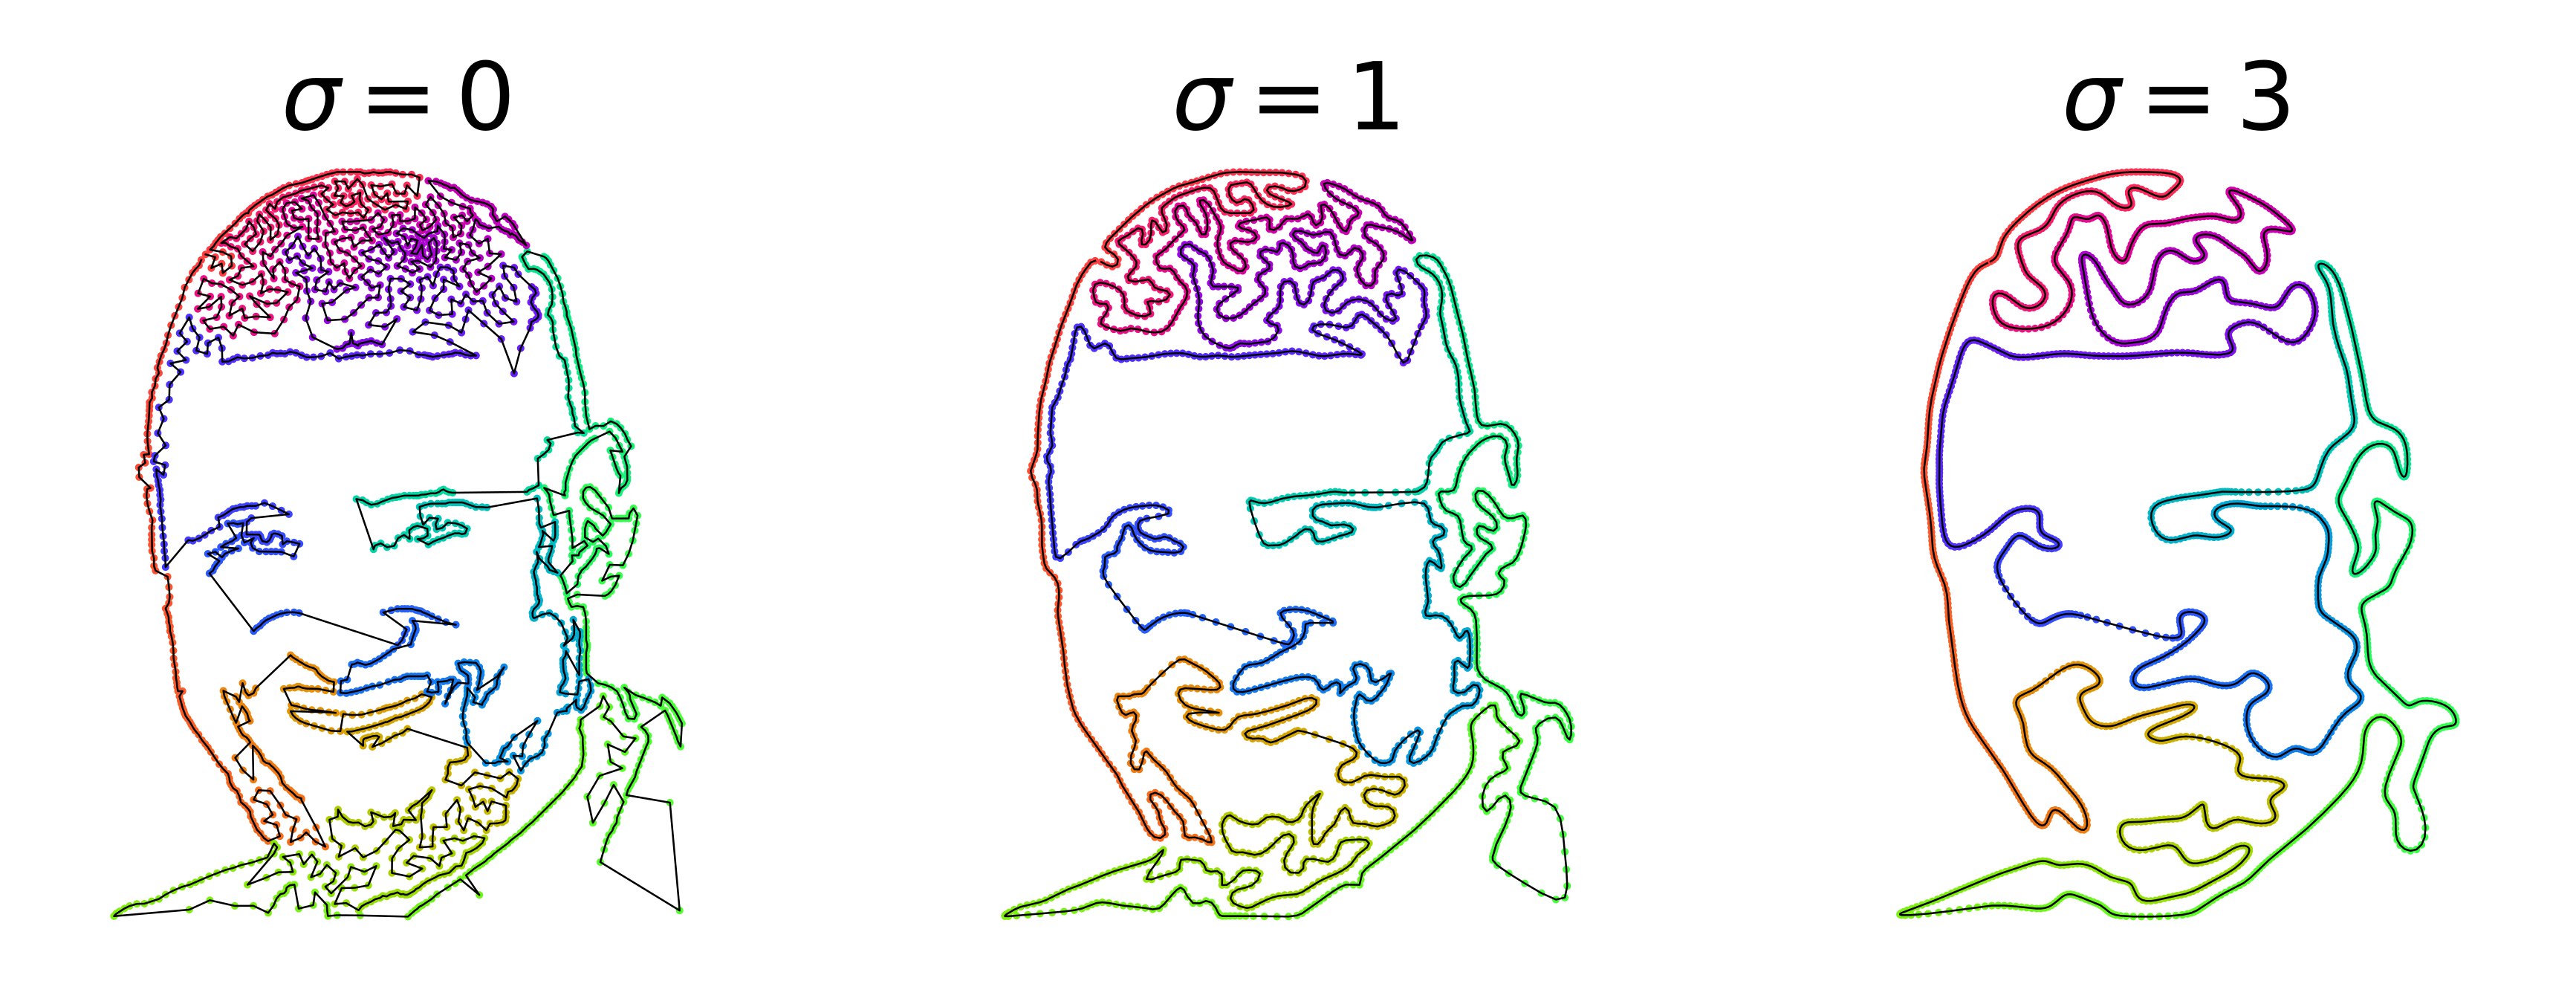
\includegraphics[width=\columnwidth]{CurvatureShortening.png}
  \caption{Anticipating that mp3 compression will introduce noise to our embedded curves, we pre-smooth them before hiding them using one application of curvature-shortening flow, which smooths the curves without introducing any crossings.  We find $\sigma=1$ to be a good tradeoff between smoothness and detail.}
  \label{fig:CurvatureShortening}
\end{figure}


Since mp3 compression introduces noise into our embedded curves, we smooth them before embedding to improve visual quality.  To this end, we apply a numerical version of curvature shortening flow described by Mokhtarian and Mackworth \cite{mokhtarian1992theory} which applies to piecewise linear curves (like our TSP tours).  The technique works by numerically by convolving coordinates of each curve with smoothed versions of Gaussians and their derivatives.  In particular, let 
\begin{equation}
  g_{\sigma}[j] = c_1 e^{-j^2 / (2 \sigma^2)}, 
  g'_{\sigma}[j] = - c_2 \frac{j}{\sigma^2} e^{-j^2 / (2 \sigma^2)}
\end{equation}

where $c_1$ and $c_2$ are appropriate normalization constants.  Then we can estimate the arc length of a sampled curve $\gamma[j]$ with the rectangular integral of a smoothed velocity estimate:

\begin{equation}
  \label{eq:arclen}
  s_{\sigma}[j] = \sum_{k=1}^j |(\gamma * g'_{\sigma})[k]|
\end{equation}

To approximately smooth a curve via one step of curvature-shortening flow, Mokhtarian and Mackworth \cite{mokhtarian1992theory} show that it suffices to first re-parameterize by the arc length $s_{\sigma}$ in Equation~\ref{eq:arclen}, and then to smooth the curve by convolving with $g_{\sigma}$.  The beauty of convolving with Gaussians as such is that $\gamma$ does not even have to be differentiable, so this works on our piecewise linear TSP tours.  Furthermore, by the Gage-Hamilton-Grayson theorem, simple curves that undergo curvature shortening flow {\em remain simple} and eventually become convex, shrinking to a point under repeated applications of the flow.  Figure~\ref{fig:CurvatureShortening} shows an example of one application of curvature shortening flow for different $\sigma$ values.



\section{Hamiltonian Paths on Watertight Triangle Meshes}
\label{sec:hamiltonian}



\section{Curve Embedding in Audio}

We now introduce our new algorithm for hiding artistic space curves, such as 2D TSP paths (Section~\ref{sec:tsp}) and 3D Hamiltonian paths (Section~\ref{sec:hamiltonian}), in audio.

\subsection{Formulation of Least Squares Problem}

Let $T = (T_1, T_2, \hdots, T_N \}$ the desired Euclidean target point sequence to hide, where each $T_i \in \mathbb{R}^d$, and $T_i[m]$ refers to the $m^{\text{th}}$ coordinate of $T_i$, and let $x$ be a set of audio samples which will serve as a carrier.  The goal is to perturb the samples of $x$ so that some function of $x$ matches $T$ as closely as possible.  The function we choose is based on a ``time regularized'' version of the magnitude Short-Time Fourier Transform (STFT) which we call a {\em sliding window sum} STFT (SWS-STFT).  As a first step, we compute a {\em non-overlapping} STFT $S$ based on a chosen window length $w$ with a total of $N$ frames:

\begin{equation}
  S_{k, j} = \sum_{n = 0}^w x_{jw + n} \left(e^{-i 2 \pi k n / w} \right) = M_{k, j} \left( e^{i P_{k, j}} \right)
\end{equation}

and we factor $S$ it into its magnitude and phase components $M$ and $P$, respectively.  Then, given a second window length $\ell$, we define the following {\em sliding window sum} function, which we apply to each row $k$ of the magnitudes of $S$ that we wish to perturb to obtain the SWS-STFT

\begin{equation}
  \text{SWS}_{\ell}\left({M_k}\right)_j = \sum_{n = 0}^{\ell-1} M_{k, j+n}
\end{equation}

The effect of $\ell$ is to smooth out the noisy time series at each row $k$ of the magnitude spectrogram so that the rows in the SW-STFT match smoother transitions in the target curves.  The resulting time series $\text{SWS}_{\ell}\left({M_k}\right)$ has $N-\ell+1$ samples.  Let's assume momentarily that $T$ has exactly this many samples; we will address the case where $len(T) > N-\ell+1$ in Section~\ref{sec:reparam}.  We seek a perturbed version of the magnitudes, $\hat{M}$ so that each coordinate $i$ is hidden in a single frequency index $k_i$ of $\hat{M}$.  To that end, we minimize the following objective function, one coordinate dimension $i = 1, ... d$ at a time:

\begin{equation}
  \label{eq:objfn}
  f_i(\hat{M}) = \sum_{j=1}^{N-\ell+1} \left( \left( \sum_{n = 0}^{\ell-1} \hat{M}_{k_i, j+n} \right) - T_i[j] \right)^2 + \lambda \sum_{j=1}^N \left( M_{k, j} - \hat{M}_{k, j} \right)^2
\end{equation}



\begin{figure}
  \centering
  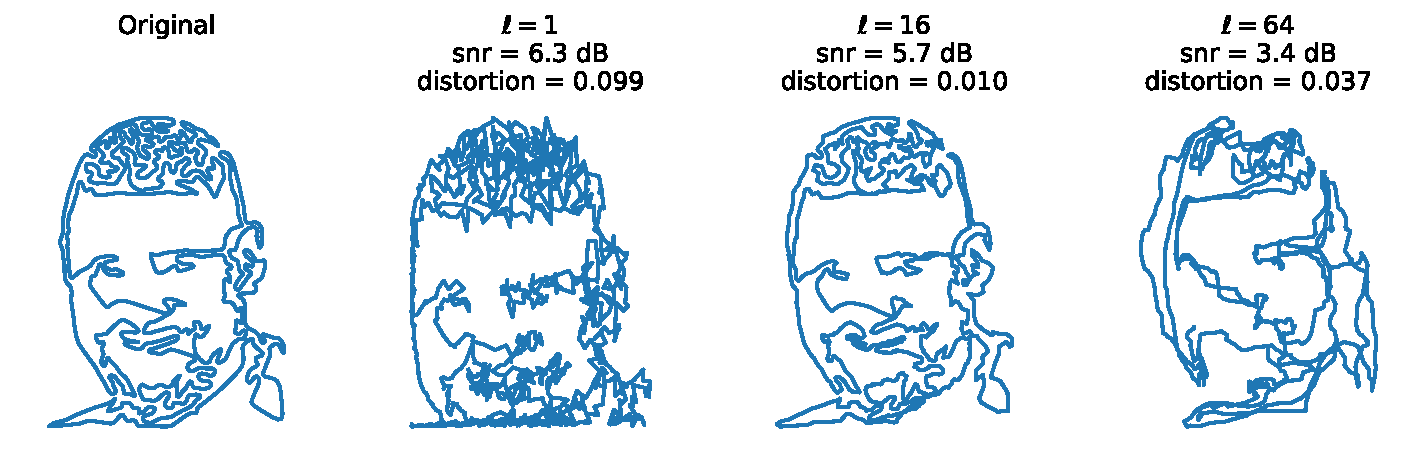
\includegraphics[width=\columnwidth]{WindowEffect.pdf}
  \caption{A larger $\ell$ for the SW-STFT in Equation~\ref{eq:objfn} leads to smoother curves which are more likely to survive mp3 encoding, but an $\ell$ that's too large can over-smooth.}
  \label{fig:WindowEffect}
\end{figure}

\begin{figure}
  \centering
  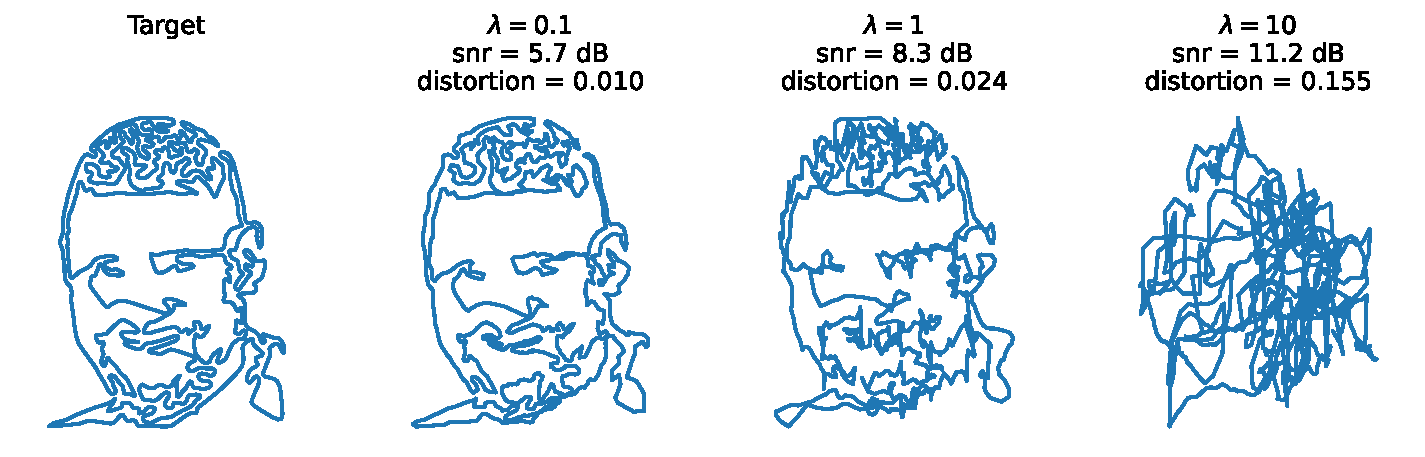
\includegraphics[width=\columnwidth]{LambdaEffect.pdf}
  \caption{A smaller $\lambda$ in Equation~\ref{eq:objfn} leads to higher geometric fidelity (Goal~\ref{goal:geomquality}), at the cost of audio quality (Goal~\ref{goal:imperceptible}), as measured by SNR.}
  \label{fig:LambdaEffect}
\end{figure}



subject to $\hat{M_{k, j}} \geq 0$.  In other words, we want the magnitude SW-STFT of a perturbed signal to match the target coordinate as well as possible, while preserving the original audio as well as possible, according to $\lambda$.  A greater $\lambda$ means that the signal will fit the original audio better, at the cost of a noisier curve.  Figure~\ref{fig:LambdaEffect} shows some examples.




\subsubsection{Efficient Computation}
\label{sec:computation}
Minimizing equation~\ref{eq:objfn} can be formulated as a sparse nonnegative linear least squares problem.  Though Equation~\ref{eq:objfn} suggest an $O(N \ell)$ time complexity to evaluate the objective function, the linear operator and its adjoint can be implemented with a number of operations proportional to $N$ only, and independent of $\ell$, using the 1D version of the ``summed area tables'' trick in computer vision \cite{lewisfast}.

It is also worth noting that a higher $\lambda$ in equation~\ref{eq:objfn} leads to a lower condition number\footnote{The condition number of a matrix is defined as the ratio of the largest to smallest singular values, and lower condition numbers are more numerically desireable.} of the matrix in the implied linear system, which leads to faster computation.  But as Figure~\ref{fig:LambdaEffect} shows, it may be worth it to use smaller $\lambda$ values.  In practice, we see it as a difference between an encoding in 30 seconds of audio that takes a few seconds for $\lambda=0.1$ versus an encoding that takes a split second for $\lambda=10$ on a CPU.



\subsubsection{The choice of non-overlapping windows}
Though some other works use transforms with overlapping windows (\cite{hwan_sik_yun_acoustic_2010,geleta_pixinwav_2021}), we find that changing different STFT bins independently can lead to STFTs that do not correspond to any real signal due to discrepancies between overlapping windows.  An algorithm like Griffin-Lim \cite{griffin1984signal} can recover a signal whose spectrogram has a locally minimal distance to the perturbed STFT, but we find that this step introduces an unacceptable level of distortion both in the target and the carrier audio.  This problem occurs even for real-valued transforms such as the Discrete Cosine Transform (which was used by \cite{geleta_pixinwav_2021}).  We sidestep this problem completely by using non-overlapping windows as in \cite{xiaoxiao_dong_data_2004}.  

The main downside of non-overlapping windows is that they lead to fewer STFT frames.  For instance, for a 30 second audio clip at 44100hz using a window length of 1024, we are limited to about 1292 frames, which is half of what we would get using an overlapping STFT with a hop length of 512.  However, a quick thought experiment shows that this is still a reasonable data rate.  Suppose that we use a sliding window length $\ell=16$, for a total of 1277 carrier samples.  Suppose also that the precision of our embedding of a 2D plane curve is roughly on par with an 8 bit per coordinate quantization in a more conventional binary encoding scheme.  Then the total number of bits transmitted over 30 seconds is $1277 \times 8 \times 2$, or about 681 bits/second.  This number jumps to about 1022 bits/second for a 3D curve.  These numbers are on part with other recent techniques that are designed to be robust to noise (e.g. 900 bits/second in the OFDM technique of \cite{eichelberger_receiving_2019}).  Furthermore, our equivalent of a ``bit error'' is additive coordinate noise,and the target can still be visible with some amount of such noise.




\subsection{Rescaling And Re-Parameterizing Targets for Better Fits}
\label{sec:reparam}


A crucial step to keep the hidden signal imperceptible is to rescale the targets to match the dynamic range of the signals.  Unfortunately, we lose relative scale information between the components, but we will explain how to store and recover this in Section~\ref{sec:componentscales}


In general, the SWS-STFT sequence $X$ will not have the same number of samples as the target $T$.  If we stick to scenarios where $T$ has more samples, we can index $X$ by a default function 



Our use of the Viterbi algorithm for re-parameterizing geometric sequences is related to the technique for corpus-based concatenative synthesis presented by the authors of \cite{schwarz2007corpus}.


As a rule of thumb, we find that having a target curve with about 1.5-2x as many samples as there are SWS-STFT frames gives enough wiggle room for the Viterbi algorithm.  Therefore, in our experiments in Section~\ref{sec:experiments}, we will generate TSP and Hamiltonian sequences with 2000 samples for our 1200-1300 SWS-STFT frames

\subsection{Storing Component Scales in Phase}
\label{sec:componentscales}

We use the technique presented by the authors of \cite{xiaoxiao_dong_data_2004} to recover the scales of each component.

\subsection{Recovering Frame Alignments}


\begin{figure}
  \centering
  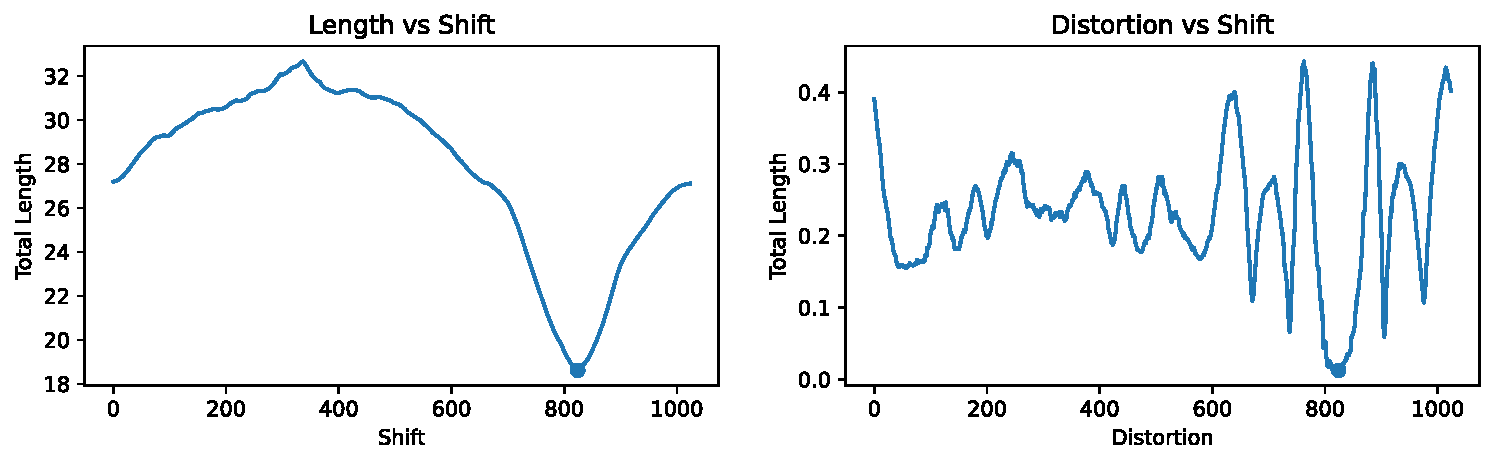
\includegraphics[width=\columnwidth]{OptimalShift.pdf}
  \caption{Curve length can be used as a proxy for distortion.}
  \label{fig:TSPTour}
\end{figure}



\section{Experiments}
\label{sec:experiments}

Below we assess the performance of our system on an extensive set of tests

Show caltech-101 and meshseg examples

\begin{figure}
  \centering
  \includegraphics[width=\columnwidth]{caltech101_samples.pdf}
  \caption{Examples of some TSP art on the Caltech-101 dataset \cite{li_andreeto_ranzato_perona_2022}.}
  \label{fig:caltech101examples}
\end{figure}

\subsection{Quantitative Metrics}

\subsection{Subjective Listening Experiment}

\begin{figure}
  \centering
  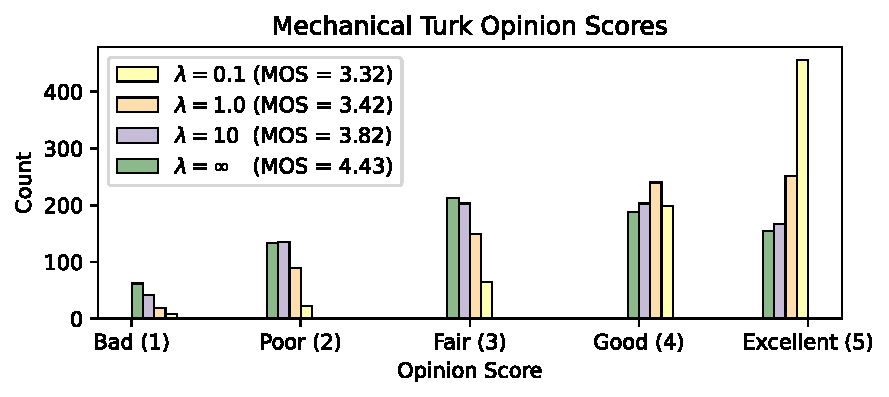
\includegraphics[width=0.8\columnwidth]{Turk.pdf}
  \caption{Results of the listening experiment on the Amazon Mechanical Turk}
  \label{fig:TurkResults}
\end{figure}


We can actually get higher SNRs using frequencies that are more audible

We ask questions similar to the authors of \cite{bassia2001robust}.

46 unique Turkers, 21 of whom participated in at least 40 rankings.

Figure~\ref{fig:TurkResults} shows the results.  Mean opinion scores are correlated with $\lambda$, but there's not much of a difference between $\lambda=0.1$ and $\lambda=1$, which suggests using the former as a rule of thumb due to its lower geometric distortion.

\section{Discussion}

%
% ---- Bibliography ----
%
% BibTeX users should specify bibliography style 'splncs04'.
% References will then be sorted and formatted in the correct style.
%
\bibliographystyle{splncs04}
\bibliography{paper}
%

\end{document}

